\chapter{Value Function Methods}
In the last two chapters, we discussed some policy gradient-based algorithms. We have also seen the fact that the policy gradient methods have high variance. Therefore, it would be nice if we could completely omit the gradient step. To achieve this, we are going to talk about the value function methods in this chapter. 

\section{An Implicit Policy}
To omit the policy gradient, one still has to generate a policy function so that it takes in a state and outputs an action. Recall in actor-critic algorithms, we use the advantage function $A^\pi(s_t,a_t)$ to gauge how much better is the action $a_t$ than the average action according to $\pi$. Provided that we have a somehow accurate representation of this advantage function, we can just forget about generating a policy $\pi$, and just do this:
$$\argmaxA_{a_t} A^\pi(s_t,a_t)$$
which means we take the best action from $s_t$, if we follow $\pi$. Even though we have no knowledge of what the policy $\pi$ actually is, by doing the $\argmaxA$, we can guarantee that the action produced is at least as good as the action from the policy function that we do not know. Therefore, as long as we have a accurate representation of the advantage function $A^\pi(s_t,a_t)$, we can implicitly generate a parameter-free policy function:
\begin{align*}
\pi'(a_t|s_t) & = \begin{cases}
                1, & \mathrm{if } \;a_t = \argmaxA_{a_t}A^\pi(s_t,a_t)\\
                 0, & \mathrm{otherwise}
                    \end{cases}
\end{align*}
and as we have shown above, this implicit policy is at least as good as the unknown policy $\pi$.

\section{Policy Iteration}
Having omitted the policy, we can then proceed to introduce the policy iteration algorithm.
\subsection{High Level Idea}
The basic idea of policy iteration algorithms is very simple: we evaluate the advantage function $A^\pi(s,a)$ and then update the policy using the update rule as defined above in the implicit policy, and then we can loop to constantly improve our policy. 

The problem here is how to evaluate $A^\pi(s,a)$. In other words, how does one find an accurate representation of the advantage function in order to accurately update the policy. As before, we have seen that the advantage function an be equivalently defined as follows:
$$A^\pi(s,a) = r(s,a) + \gamma\mathbb{E}\left[V^\pi(s')\right]-V^\pi(s)$$
Therefore, if we can evaluate the value function $V^\pi(s)$ then we can also evaluate $A^\pi(s,a)$. So in the high-level policy iteration algorithm, we can just use the value function in place of the advantage function.

\subsection{Dynamic Programming}
Now let us make a simple assumption. Suppose we know a priori the transition probability $p(s'|s,a)$ and both states $s$ and action $a$ are discrete. Then a very natural dynamic programming update is the bootstrapped update, as we have seen before:
$$V^\pi(s)\leftarrow \mathbb{E}_{a\sim\pi(a|s)} \left[r(s,a) + \gamma\mathbb{E}_{s'\sim p(s'|s,a)}\left[V^\pi(s')\right]\right]$$
and we can just use the current estimate inside the nested expectation for simplicity. 

According to our definition of the implicit policy function $\pi'$, the policy is actually deterministic. Therefore, we can completely get rid of the outside expectation, and the value function update can be further simplified as:
$$V^\pi(s)\leftarrow r(s,\pi(s)) + \gamma\mathbb{E}_{s'\sim p(s'|s,a)}\left[V^\pi(s')\right]$$
\begin{algorithm}[t!]
\caption{Policy Iteration via DP}
\begin{algorithmic}[1]
\label{alg:policyiter1}
\WHILE{true}
    \STATE Evaluate $V^\pi(s,a)$
    \STATE Set $\pi\leftarrow \pi'$
\ENDWHILE
\end{algorithmic}
\end{algorithm}
This version of policy iteration is sketched in Algorithm \ref{alg:policyiter1}

We can even further simplify the dynamic programming update. Note that we in each iteration, we are updating the policy first in order to update the value function. Thus, it would be faster if we could skip the policy part and directly improve the value estimation. Meanwhile, the $\argmaxA$ operation that we apply on the advantage function itself is an implicit policy. We also know that $\argmaxA_{a_t}A^\pi(s,a) = \argmaxA_{a_t}Q^\pi(s,a)$, because the two values only differ by the subtraction term $V^\pi$, which does not depend on action:
$$A^\pi(s,a) = r(s,a) + \gamma\mathbb{E}\left[V^\pi(s')\right]$$
\begin{algorithm}[t!]
\caption{Value Iteration via DP}
\begin{algorithmic}[1]
\label{alg:policyiter2}
\WHILE{true}
    \STATE Set $Q(s,a)\leftarrow r(s,a) + \gamma\mathbb{E}\left[V(s')\right]$
    \STATE Set $V(s) \leftarrow \max_{a}Q(s,a)$
\ENDWHILE
\end{algorithmic}
\end{algorithm}
Having this, we can simplify the policy iteration algorithm further, as illustrated in Alg. \ref{alg:policyiter2}. As we skipped the policy update part, we call this new, simplified algorithm ``value iteration algorithm''.

\section{Fitted Value Iteration}
The policy iteration and value iteration algorithm we discussed above are heavily based on an impractical assumption: the total number of states is finite and small, because we are trying to construct a tabular expression of the value function and the Q function. Apparently, the tables are going to explode in dimensions if there are a lot of states. We call this the Curse of Dimensionality. To resolve this problem, we can use a neural network to approximate the functions instead of constructing a tabular expression of the function. 

\subsection{Fitted Supervised Value Iteration Algorithm}
Since we know that the value function is defined as $\max_a Q^\pi(s,a)$, we can use this definition as the labels for the value function in order to define a L2 loss function:
$$\mathcal{L}(\phi) = \frac{1}{2}\lvert|V_\phi(s) - \max_{a}Q^\pi(s,a)|\rvert^2$$
\begin{algorithm}[t!]
\caption{Fitted Value Iteration}
\begin{algorithmic}[1]
\label{alg:fittedvaliter}
\WHILE{true}
    \STATE set $y_i \leftarrow \max_{a_i}\left(r(s_i,a_i) + \gamma \mathbb{E}\left[V_\phi(s'_i)\right]\right)$
    \STATE set $\phi \leftarrow \argminA_\phi \frac{1}{2}\Sigma_i\lvert|V_\phi(s_i) - y_i|\rvert^2$
\ENDWHILE
\end{algorithmic}
\end{algorithm}
Then we can sketch out a simple fitted value iteration algorithm using this loss function in Algorithm \ref{alg:fittedvaliter}. Note that when setting the label, the ideal step to take is to enumerate all the states and find the corresponding label. However, when it is impractical, one could just use some samples and enumerate all the actions to find the labels. Moreover, when we take the maximum over all the actions from a state, we implicitly assume that the transition dynamics are known. Why? Because we want to take an action, record the value of that action, and then roll back to the previous state in order to check the values of other actions. Thus, without the transition dynamics, we cannot easily take the maximum.
\subsection{Fitted Q-Iteration Algorithm}
To address this problem, we can apply the same ``max'' trick in policy iteration. In policy iteration, we skip the policy update and calculate the values directly. Here in fitted value iteration, we can get around the transition dynamics by looking up the Q function table, because $V_\phi(s) \simeq \max_{a}Q_\phi(s,a)$, and this max operation is merely a table lookup from the Q value table. Consequently, we are now iterating on the Q values. Such a method works for off-policy samples (unlike actor-critic), and it only needs one network, so it does not have any high-variance policy gradient. However, as we shall see in later sections, such methods do not have convergence guarantees on non-linear functions, which could potentially be problematic.

The full fitted Q-iteration algorithm is shown in Algorithm \ref{alg:fittedQ}.
\begin{algorithm}[t!]
\caption{Fitted Q-Iteration Algorithm}
\begin{algorithmic}[1]
\label{alg:fittedQ}
\REQUIRE Some base policy for data collection; hyperparameter $K$
\WHILE{true}
    \STATE Collect dataset $\{(s_i,a_i,s'_i,r_i)\}$ using some policy
    \FOR{$K$ times}
        \STATE Set $y_i\leftarrow r(s_i,a_i) + \gamma \max_{a'_i}Q_\phi(s'_i,a'_i)$
        \STATE Set $\phi \leftarrow \argminA_\phi \frac{1}{2}\Sigma_i\lvert|Q_\phi(s_i,a_i) - y_i|\rvert^2$
    \ENDFOR
\ENDWHILE
\end{algorithmic}
\end{algorithm}
\subsection{A Closer Look at Q-Iteration Algorithm}
Let us take a closer look at the fitted Q-learning algorithm. 
First, let us discuss why the algorithm is fully off-policy. In step 2 of Alg. \ref{alg:fittedQ}, we are not collecting a lot of transition data, and we do not care about the trajectories. Furthermore, in step 4, we are taking the step off-policy in that we do not care about which state we are going to, because we only care about the value of the transition. In other words, the tansition we take is independent of the unknown policy $\pi$. Therefore, the fitted Q-iteration algorithm is fully off-policy.

Another question we can ask is that what is fitted Q-iteration actually optimizing? In step 5 of Alg. \ref{alg:fittedQ}, we are minimizing the difference between the Q function value and the label we approximated. In fact, we call this difference the Bellman Error, defined as follows:
$$\epsilon = \frac{1}{2}\mathbb{E}_{(s,a)\sim\beta}\left[\left(Q_\phi(s,a) - \left[r(s,a)+\gamma\max_{a'}Q_\phi(s',a')\right]\right)^2\right]$$
So in this particular step, we are optimizing the Bellman Error, and if $\epsilon = 0$, we have optimal Q-function, corresponding to optimal policy $\pi$, which can be recovered by the $\argmaxA$ operation. However, rather ironically, we do not know what we are optimizing in the previous steps, and this is a potential problem of the fitted Q-learning algorithm, and most convergence guarantees are lost when we do not have the tabular case.

\subsection{Online Q-Iteration Algorithm}
We can also make the samples more efficient by making the Q-iteration algorithm completely online. By online we mean that we do not store any transition. Instead, we take one transition and immediately apply the transition to our value update. The online version of Q-Iteration Algorithm is sketched in Alg. \ref{alg:onlineQiter}.
\begin{algorithm}[t!]
\caption{Online Q-Iteration Algorithm}
\begin{algorithmic}[1]
\label{alg:onlineQiter}
\WHILE{true}
    \STATE Take some action $a_i$ and observe $(s_i,a_i,s'_i,r_i)$
    \STATE $y_i = r(s_i,a_i) + \gamma \max_{a'}Q_\phi(s_i,a_i,s'_i,r_i)$
    \STATE $\phi \leftarrow \phi-\alpha\frac{dQ_\phi}{d\phi}(s_i,a_i)(Q_\phi(s_i,a_i) - y_i)$
\ENDWHILE
\end{algorithmic}
\end{algorithm}
As we see in step 2 of the algorithm, we are taking an action off-policy, so we have a lot of choices to make. 

\section{Value Function Learning Theory}
One question that one might ask after seeing the variety of algorithm as shown above is does the value function method converge? If so, it converges to what? To take a closer look in order to answer the question, let us define a Bellman backup operator $\mathcal{B}$:
$$\mathcal{B}V = \max_a r_a + \gamma\mathcal{T}_aV$$
where $r_a$ is a stacked vector of rewards at all states for action $a$. $\mathcal{T}_a$ is a matrix of transitions for action $a$ such that $\mathcal{T}_{a,i,j} = p(s'=i|s=j, a)$.
We also define a fixed point of the Bellman backup operator $\mathcal{B}$, denoted as $V^*$:
$$V^*(s) = \max_a r(s,a) + \gamma\mathbb{E}[V^*(s')]$$
so it is similar to the notion of the stationary distribution in MDP, $V^* = \mathcal{B}V^*$. One can prove that such fixed point always exists, and it corresponds to the optimal policy, but the online question is: will we reach it?

In the \textbf{tabular representation} case, we can prove that value iteration always reaches the fixed point $V^*$ because mathematically, the Bellman backup operator is a \textbf{contraction}. A contraction in our scenario is defined as follows: for any $V$ and $\Bar{V}$, we have $\lvert|\mathcal{B}V - \mathcal{B}\Bar{V}|\rvert_\infty \leq \lvert|V -\Bar{V}|\rvert_\infty$. In other words, after applying the Bellman backup operator, the gap always gets smaller by $\gamma$ with respect to the l-$\infty$ norm.

Now let us proceed to analyze the \textbf{non-tabular representation} case. In this scenario, unfortunately, we have lost a lot of convergence guarantees. Recall that in normal value iteration (tabular case), we use the Bellman backup operator $\mathcal{B}$ to update $V$: $V\leftarrow \mathcal{B}V$. In fitted (non-tabular) value iteration, we use the Bellman backup operator, $\mathcal{B}$, together with another operator $\Pi$. The operator $\Pi$ is defined as:
$\Pi V = \argminA_{V'\in\Omega}\frac{1}{2}\sum\lvert|V'(s) - V(s)|\rvert^2$. So $\Pi$ is a projection onto $\Omega$ in terms of l2 norm. This projection is illustrated in Fig. \ref{fig:bellmanbackup}. The set that $V$ and $V'$ lie in can be thought as a representation of all value functions. Therefore, the set $\Omega$ can be represented by neural networks.

\begin{figure}
    \centering
    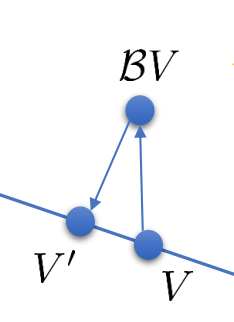
\includegraphics[scale=0.5]{figures/bellmanbackup.png}
    \caption{Bellman Backup Projection}
    \label{fig:bellmanbackup}
\end{figure}

Now we have the two operators defined, we can see that $\mathcal{B}$ is a contraction with respect to the l-$\infty$ norm, and the operator $\Pi$ is a contraction with respect to the l2 norm. But what if we impose one operator to another? Is the compound operator also a contraction? The answer is no. Therefore, such non-tabular Q-iterations do not have any convergence guarantee as the operator is not a contraction. 

What about fitted Q-iteration? Concisely, the fitted Q-iteration algorithm can be defined as $Q \leftarrow \Pi\mathcal{B}Q$. Therefore, the same reasoning can be applied to the fitted Q-learning: since the compound operator is no longer a contraction, we do not have any guarantee for convergence. We can say the same thing in online Q-iteration as well.

However, one might ask, in step 4 of Alg. \ref{alg:onlineQiter}, aren't we just doing gradient descent, which definitely converges? As a matter of fact, this is not real gradient descent in that the target value is constantly changing due to the off-policy nature of this algorithm. So we have this sad corollary: in general cases, fitted bootstrapped policy evaluation does not converge.